\chapter{Problématique de la détection}
	\section{Généralités}

Les techniques de comparaisons d'organes de décision types ROC (Receiver-Operating Curve) proviennent à l'origine du domaine des télécommunications. Il fallait une métrique permettant de tester les performances des systèmes RADAR\cite{zou2007receiver}. \todo{??}

Les courbes ROC servent donc à évaluer la capacité de un ou plusieurs ``observateurs'' à discriminer deux classes. On utilise habituellement les informations de sensibilité et de spécificité pour l'évaluation

Les techniques que j'ai utilisé par la suite pour comparer les performances des algorithmes de correction du mouvement respiratoire sont basées sur les courbes ROC, ou Receiver-Operating Curves.

Les courbes ROC ont été utilisées en médecine à partir de ... (1978 publi FROC)

La \emph{sensibilité} (eq. \ref{eq:sensib}) correspond à la proportion d'images correctement évaluées pathologiques par l'observateur par rapport au nombre total d'images réellement pathologiques. Elle donne une information sur la capacité du classifieur à détecter les cas pathologiques.

\begin{equation}
	\label{eq:sensib}
	Sensibilite = \frac{VP}{VP + FN}
\end{equation}

La \emph{spécificité} (eq. \ref{specif}) représente le même type de grandeur, mais cette-fois ci appliquée aux cas non pathologiques : elle correspond à la capacité du test à donner un résultat négatif lorsque l'image est non pathologique.

\begin{equation}
	\label{eq:specif}
	Specificite = \frac{VN}{VN + FP}
\end{equation}

Ces deux grandeurs sont complémentaires mais ne permettent pas à elle seules de comparer des classifieurs. En effet, en pratique clinique, 

	\section{Méthodologie ROC Receiver-Operating Curve}

Les ROC sont des courbes indiquant la spécificité et la sensibilité du modèle de classification pour différents niveaux de certitudes.

\todo{include description type Sandrine}

l'évaluation d'un observateur par la méthode ROC implique de créer un jeu de données de données labellisé en deux classes : Normale (H0) et Pathologiques (H1). L'observateur va se voir présenter l'ensemble des images et devra décide pour chacune si elle est H1 ou H0. Cela se fait en donnant une note : plus elle sera élevée, plus l'observateur va considérer qu'il est en présence d'un cas pathologique. A l'inverse, une note basse va indiquer un cas sain.

Le problème de cette technique est que l'observateur n'est aps obligé de donner une information de localisation du problème dans l'image. Dans notre cas, nous voulons comparer des classifieurs qui détectent les tumeurs dans l'image. Il faut non seulement savoir si des lésions sont présentes, mais aussi avoir leur nombre et leur localisation. Cela est plus proche du travail en routine clinique qui consiste à évaluer l'étendue et le nombre des lésions pour déterminer l'efficacité d'un traitement par exemple. 

Pour éviter cette limitation, plusieurs extensions à la méthodologie ROC sont décrites dans la littérature. Celle qui correspond le plus à nos besoins (multi site, multi lésions) est la courbe Free-ROC.

Les courbes ROC permettent de choisir le seuil optimal pour 

	\section{Free-ROC}	

les courbes Free-ROC sont une généralisation des courbes ROC aux cas où l'observateur ne connaît à priori ni le nombre ni la localisation des lésions dans l'image. Il doit indiquer un ensemble de lésions potentielles dans l'image et associer à chacune une note.

Dans ce cas, on ne peut pas utiliser le formalisme ROC car le terme de specificité n'est pas directement utilisable. On utilise en fait directement le nombre moyen de faux positifs par image pour un seuil donné.


\begin{figure}[h]
	
	\label{fig:courbeFROC}
	\begin{center}
	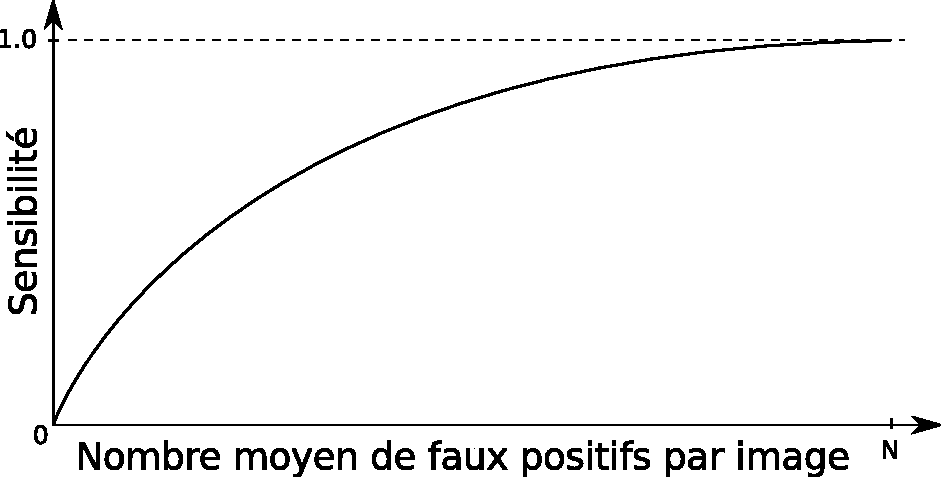
\includegraphics[width=10cm]{images/FROC}
	\end{center}
	\caption{Courbe F-ROC}
\end{figure}



\chapter{Systèmes de détection}

	\section{Les CAD en TEP}


	\section{Types de classification}
		\subsection{supervisée - méthodologie}

Les classifieurs supervisés nécessitent une connaissance a priori des classes. On entraîne le classifieur en lui fournissant des \emph{exemples} de cas avec l'étiquette associée. A partire de cette base de données d'entraînement, le classifieur va générer un \emph{modèle} predictif permettant de classer de futurs exemples non encore connus.


		\subsection{non supervisée - méthodologie}

Dans le système de classificatio non supervisé, on fourni directement au classifieur l'ensemble des données à traiter. Il devra de lui-même discerner 
	\section{classifieurs}

		
		\subsection{SVM (Separateur à Vaste Marge)}

Ce type de classifieur se base sur 
		\subsection{LDA}

	\section{Systèmes humain}
	% besoin d'avoir des données fiables ?